\documentclass{protokol}
\leftheader{Charakteristiky optoel. součástek}
\centerheader{Praktikum III}
\rightheader{Tomáš Derner}

\begin{document}

  \section*{Úkol}

    \begin{enumerate}
      \item Na internetu najděte katalogové listy všech optoelektronických součástek, které budete v úloze používat, konkrétní měřené součástky vybere vyučující. Parametry důležité ke splnění pracovních úkolů vypište a přiložte do zápisu z měření.
      \item Změřte voltampérové a světelné charakteristiky dvou luminiscenčních diod v propustném směru. Grafy vytvořte v praktiku, jsou povinnou součástí zápisu z měření.
      \item Ze změřených V-A charakteristik určete pro jednotlivé diody statický odpor $R_d$, dynamický odpor $R_{di}$, hodnotu konstanty n a prahové napětí $U^*$. Určete, z jakého materiálu jsou jednotlivé diody zhotoveny. Nezapomeňte na graf $\ln(I_F)$ vs. $U_F$.
      \item Změřte charakteristiky fototranzistoru při třech různých hladinách osvětlení. Měření proveďte pomocí pikoampérmetru s vestavěným zdrojem Keithley s funkcí ukládání dat do paměti přístroje. Povinnou součástí zápisu z měření jsou grafy naměřených charakteristik, tabulky do protokolu netiskněte.
      \item Změřte zisk fototranzistoru.
    \end{enumerate}

  \section*{Teorie}

    Optoelektronické součástky využívají fyzikální vlastnosti polovodičových P-N přechodů. V této úloze studujeme luminiscenční diody, fotodiody a fototranzistor.

    Luminiscenční diody LED jsou založeny na emisi fotonů z oblasti P-N přechodu, kterým prochází proud. Voltampérové charakteristiky těchto součástek záleží mimo jiné na geometrii, vlastnostech přechodu a použitém materiálu.

    Pro LED diody definujeme sériový statický odpor v pracovním bodě $U_{F_0}$, $I_{F_0}$ jako 
    \begin{equation}
      R_d = \frac{U_{F_0}}{I_{F_0}}.
    \end{equation}
    Můžeme ho určit lineární regresí lineární části VA závislosti.

    Sériový dynamický odpor spočítáme pomocí
    \begin{equation} \label{eq:R_di}
      R_{di} = R_d \frac{n k T}{e U_{F_0}},
    \end{equation}
    kde $k$ je Boltzmannova konstanta, $T$ absolutní teplota, $e$ náboj elektronu a $n$ bezrozměrná konstanta popisující výše jmenované vlivy na průběh VA charakteristiky diody.
    
    Tuto konstantu spočteme podle vztahu
    \begin{equation} \label{eq:n}
      n = \frac{e}{kT} \frac{U_{F_1} - U_{F_2}}{\ln \frac{I_{F_1}}{I_{F_2}}}.
    \end{equation}

    Prahové napětí $U^*$ je takové napětí, při kterém dochází ke zlomu v lineárním průběhu VA charakteristiky, viz \cite{teorie}.

    Fotodiody a fototranzistory fungují na principu opačném k principu LED diod. Fotony o vhodné energii dopadají na P-N přechod a vyvolávají vznik elektrického napětí na jeho vývodech. Fototranzistory se používají pro detekci slabších světelných toků, pro které není fotodioda dostatečně citlivá.

    V režimu užívaném v tomto praktiku je závislost fotoelektrického proudu $I_\Phi$ fotodiodou na světelném toku v širokém rozsahu lineární, kvalitativní vlastnosti se tedy dají usuzovat z průběhu $I_\Phi$. Světelnou charakteristikou LED diody proto v tomto praktiku nazýváme závislost fotoelektrického proudu $I_\Phi$ detektoru na proudu $I_F$ protékajícím diodou.

    Při zapojení fototranzistoru popsaném v návodu \cite{navod} je fotoelektrický proud v kolektoru $I_{C0}$ dán přibližným vztahem 
    \begin{equation}
      I_{C0} = G I_\Phi,
    \end{equation}
    kde G je zisk fototranzistoru a $I_\Phi$ je primární fotoproud, který získáme zkratováním emitoru s bází.

    Voltampérovými charakteristikami fototranzistoru se rozumí závislost $I_{C0}$ na napětí mezi kolektorem a emitorem $U_{CE}.$ Mění se v závislosti na dopadajícím světelném toku.

  \section*{Výsledky}

    \subsection*{Úkol 2}

      Byly měřeny dvě LED diody, červená \textbf{LQ1131} a modrá \textbf{560LB7D}. Všechny hodnoty byly měřeny automaticky multimetrem \textbf{Keithley 6487} s automatickým nastavením rozsahu. Chyby měřicího přístroje nejsou signifikantní vedle chyb lineárních regresí.

      Voltampérové charakteristiky zobrazují grafy \ref{fig:red} a \ref{fig:blue}, světelné charakteristiky grafy \ref{fig:red_svet} a \ref{fig:blue_svet}.

    \subsection*{Úkol 3}

      Převrácením směrnic lineárních regresí v grafu \ref{fig:red} a \ref{fig:blue} byla získána hodnota sériového statického odporu červené resp. modré diody
      $$ R_d^\textit{č} = \SI{14.77 \pm 0.20}{\ohm}, $$
      $$ R_d^m = \SI{17.17 \pm 0.17}{\ohm}. $$

      Lineární regresí v grafu \ref{fig:red_log} a \ref{fig:blue_log} a použitím vztahu \eqref{eq:R_di} a \eqref{eq:n} získáme pro $U_{F_0}$ odpovídající proudu $\SI{20}{mA}$ hodnoty sériového dynamického odporu
      $$ R_{di}^\textit{č} = \SI{0.399 \pm 0.008}{\ohm},$$
      $$ R_{di}^m = \SI{0.289 \pm 0.010}{\ohm}.$$

      Z lineární regrese v grafech \ref{fig:red} a \ref{fig:blue} byly určeny hodnoty 
      $$ U_\textit{č}^* = \SI{1.55 \pm 0.03}{V}, $$
      $$ U_m^* = \SI{2.77 \pm 0.04}{V}. $$


    \begin{figure}[H]
      \centering
      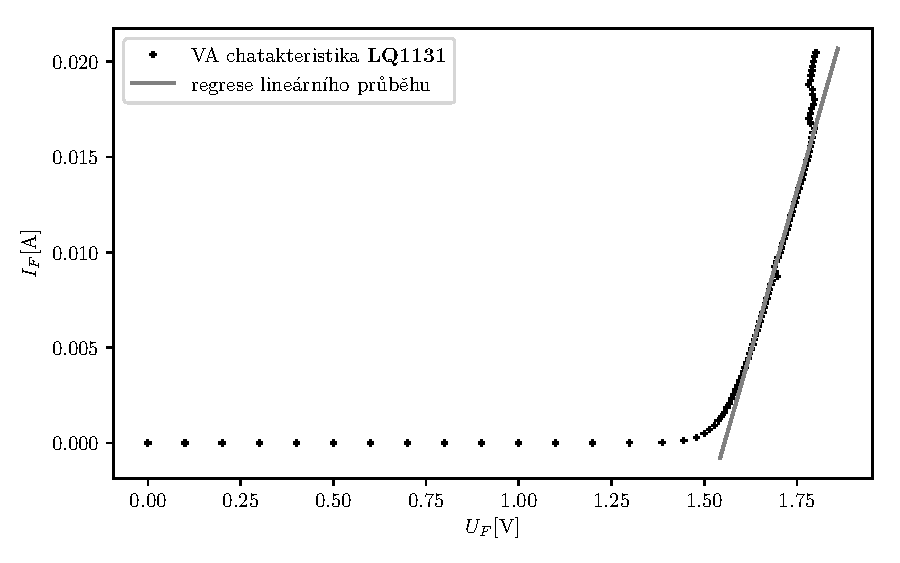
\includegraphics[]{red}
      \caption{Graf voltampérové charakteristiky diody \textbf{LQ1131}}
      \label{fig:red}
    \end{figure}

    \begin{figure}[H]
      \centering
      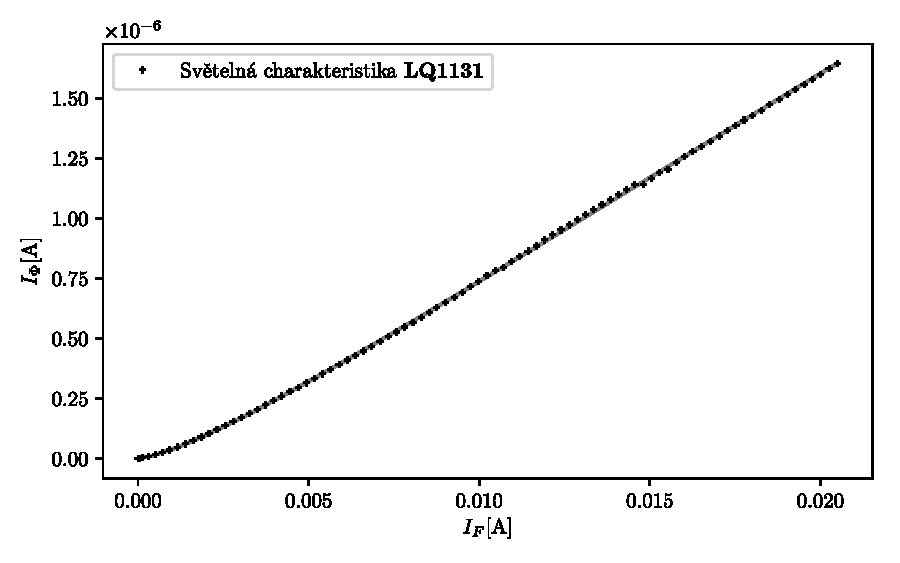
\includegraphics[]{red_svet}
      \caption{Graf světelné charakteristiky diody \textbf{LQ1131}}
      \label{fig:red_svet}
    \end{figure}

    \begin{figure}[H]
      \centering
      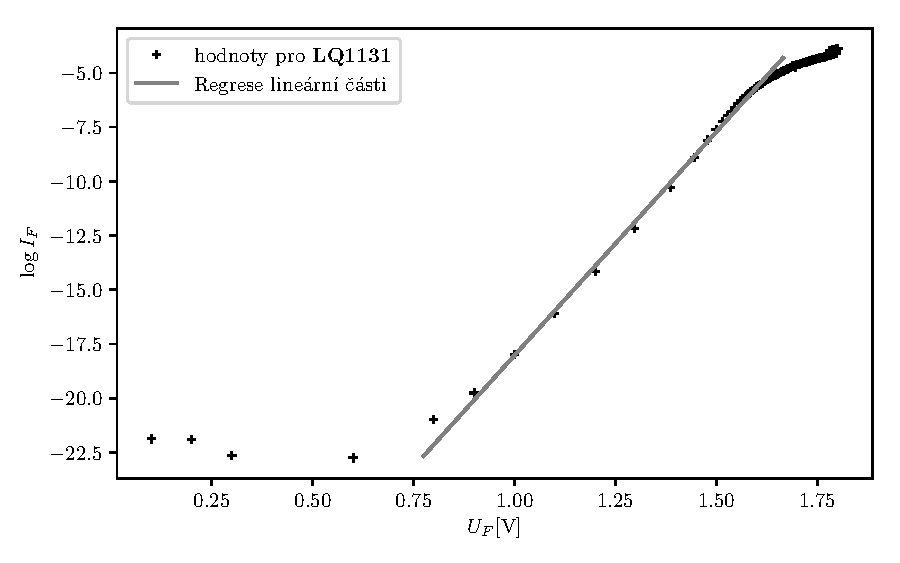
\includegraphics[]{red_log}
      \caption{Závislost $\log{I_F}$ na $U_F$ pro diodu \textbf{LQ1131}}
      \label{fig:red_log}
    \end{figure}

    \begin{figure}[H]
      \centering 
      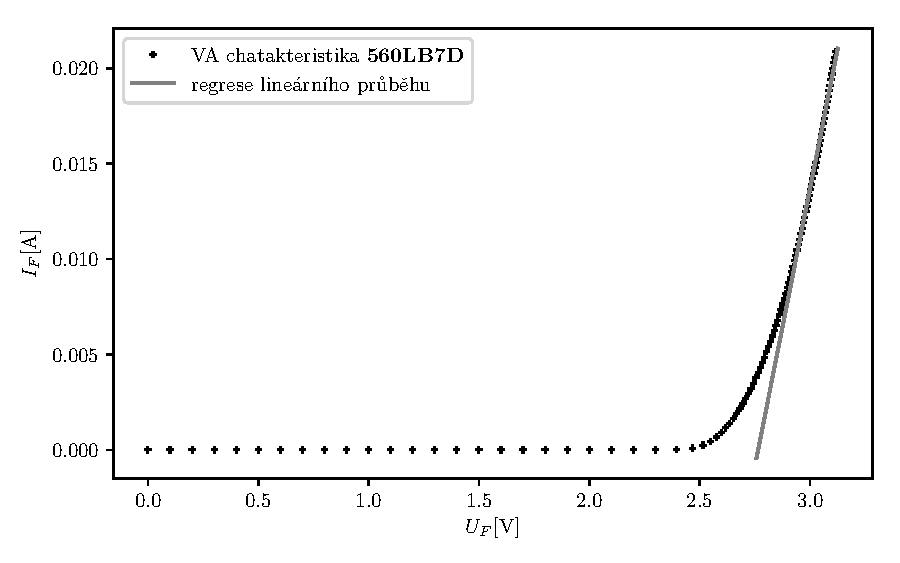
\includegraphics[]{blue}
      \caption{Graf voltampérové charakteristiky diody \textbf{560LB7D}}
      \label{fig:blue}
    \end{figure}

    \begin{figure}[H]
      \centering
      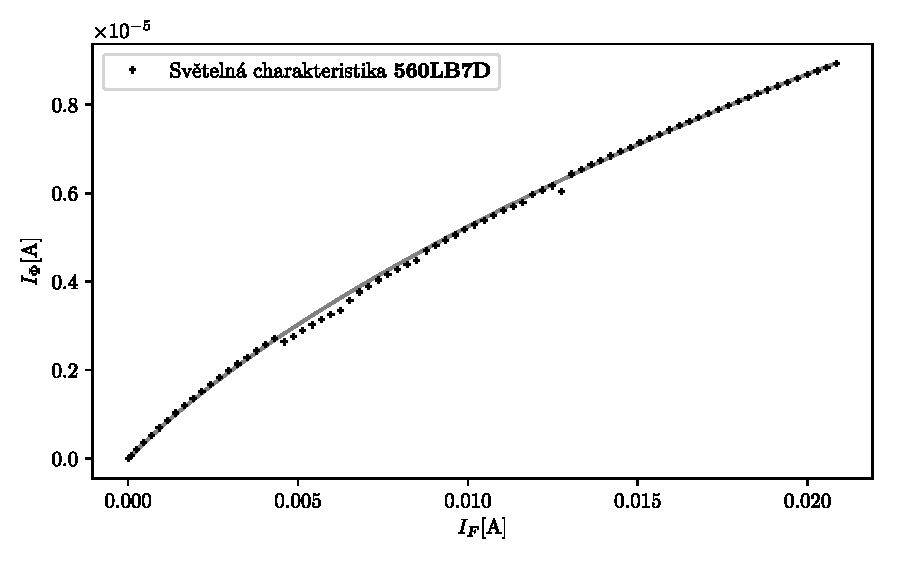
\includegraphics[]{blue_svet}
      \caption{Graf světelné charakteristiky diody \textbf{560LB7D}}
      \label{fig:blue_svet}
    \end{figure}

    \begin{figure}[H]
      \centering
      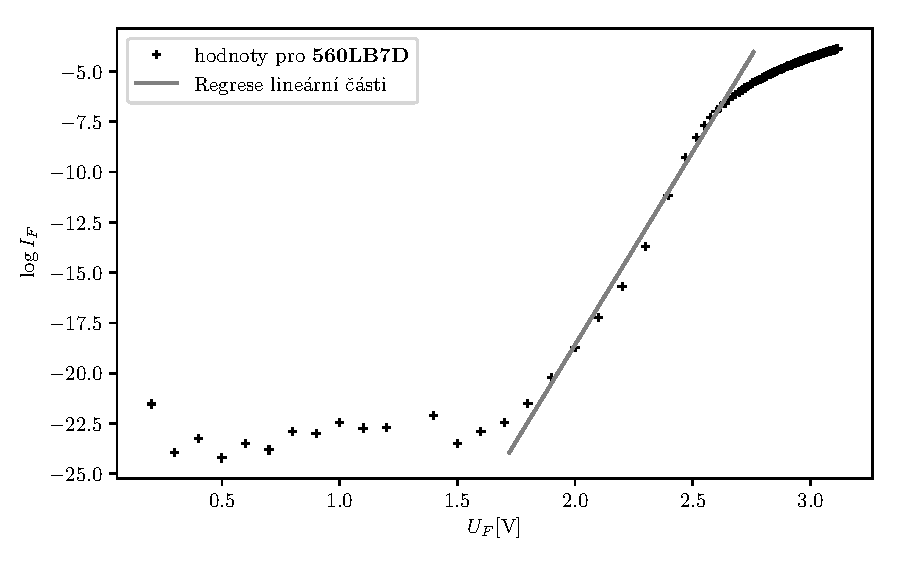
\includegraphics[]{blue_log}
      \caption{Závislost $\log{I_F}$ na $U_F$ pro diodu \textbf{560LB7D}}
      \label{fig:blue_log}
    \end{figure}

    \subsection*{Úkol 4}

      Následující graf zobrazuje voltampérové charakteristiky fototranzistoru pro osvětlení způsobené proudem $I_F$ protékajícím LED diodou.

    \begin{figure}[H]
      \centering
      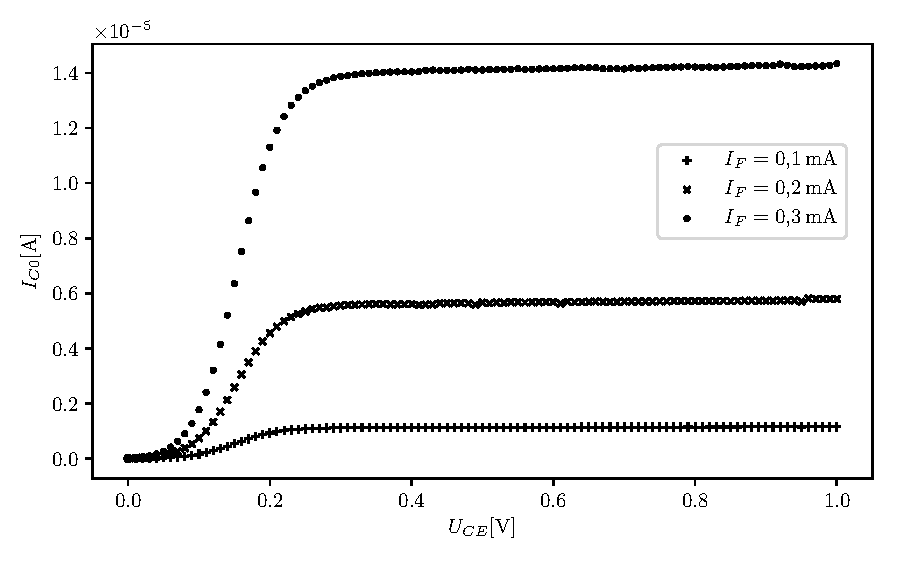
\includegraphics[]{fototr}
      \caption{VA charakteristiky fototranzistoru při různých proudech LED diodou}
      \label{fig:fototr}
    \end{figure}

    \subsection*{Úkol 5}

      Pro získání zisku fototranzistoru byly měřeny hodnoty $I_{C0}$ a $I_\Phi$ při napětí mezi kolektorem a emitorem $U_{CE} = \SI{3}{V}$. Chyby byly odhadnuty z proměnnosti údajů zobrazených na displeji (měřicí přístroj má výrazně větší přesnost).

      Při osvětlení fototranzistoru diodou protékanou proudem $\SI{0.1}{mA}$ byly naměřeny hodnoty 
      $$ I_\Phi^{\SI{0.1}{mA}} = \SI{8.0 \pm 0.3}{nA}, $$
      $$ I_{C0}^{\SI{0.1}{mA}} = \SI{1.14 \pm 0.01}{\micro\ampere}. $$
      Zisk je pak 
      $$ G^{\SI{0.1}{mA}} = \num{143 \pm 6}. $$

      Při osvětlení fototranzistoru diodou protékanou proudem $\SI{0.2}{mA}$ byly naměřeny hodnoty 
      $$ I_\Phi^{\SI{0.2}{mA}} = \SI{29.8 \pm 0.3}{nA}, $$
      $$ I_{C0}^{\SI{0.2}{mA}} = \SI{5.14 \pm 0.05}{\micro\ampere}. $$
      Zisk je pak 
      $$ G^{\SI{0.2}{mA}} = \num{172 \pm 2}. $$

      Při osvětlení fototranzistoru diodou protékanou proudem $\SI{0.3}{mA}$ byly naměřeny hodnoty 
      $$ I_\Phi^{\SI{0.3}{mA}} = \SI{64.2 \pm 0.2}{nA}, $$
      $$ I_{C0}^{\SI{0.3}{mA}} = \SI{14.20 \pm 0.05}{\micro\ampere}. $$
      Zisk je pak 
      $$ G^{\SI{0.3}{mA}} = \num{221 \pm 1}. $$

  \section*{Diskuse}

    Mnoho veličin a jejich chyb naměřených v tomto praktiku bylo určeno pomocí lineárních regresí. Protože však měřené průběhy nebyly v celém rozsahu lineární, do zpracování dat vstupuje jistý subjektivní prvek výběru lineární části závislosti pro regresi, tato dodatečná chyba je však jen těžko systematicky zachytitelná. Zároveň jsou u těchto veličin zanedbány chyby způsobené nepřesností měřicího přístroje, které jsou však bez výjimky řádově menší, než chyby lineárních regresí, tudíž by se stejně neprojevily.

    Naměřené voltampérové a světelné charakteristiky jakožto i voltampérové charakteristiky vesměs odpovídají teoretickým předpovědím. Je však nutné podotknout, že napříč měřeními se v závislostech nekonzistentně vyskytují drobné nespojitosti a výchylky (viz pravá část grafu \ref{fig:red} či část grafu \ref{fig:blue_svet}), které neumíme uspokojivě vysvětlit.

  \section*{Závěr}

    Naměřené voltampérové a světelné charakteristiky dvou LED diod i voltampérové charakteristiky fototranzistoru kvalitativně odpovídají teoretickým průběhům.

    Sériové statické odpory diod jsou
    $$ R_d^\textit{č} = \SI{14.77 \pm 0.20}{\ohm}, $$
    $$ R_d^m = \SI{17.17 \pm 0.17}{\ohm}, $$
    sériové dynamické odpory
    $$ R_{di}^\textit{č} = \SI{0.399 \pm 0.008}{\ohm},$$
    $$ R_{di}^m = \SI{0.289 \pm 0.010}{\ohm}.$$

    Prahová napětí jsou 
    $$ U_\textit{č}^* = \SI{1.55 \pm 0.03}{V}, $$
    $$ U_m^* = \SI{2.77 \pm 0.04}{V}. $$

    Zisk fototranzistoru je pro tři hodnoty proudu diodou
    $$ G^{\SI{0.1}{mA}} = \num{143 \pm 6}, $$
    $$ G^{\SI{0.2}{mA}} = \num{172 \pm 2}, $$
    $$ G^{\SI{0.3}{mA}} = \num{221 \pm 1}. $$

  \begin{thebibliography}{}

    \bibitem{teorie}
    Studijní text "Kvantová optika a optoelektronika", dostupné z \\ \url{http://physics.mff.cuni.cz/vyuka/zfp/_media/zadani/texty/txt_305.pdf}, 9.\,3.\,2018
    \bibitem{navod}
    Návod "Pokyny k měření pikoampérmetrem", dostupný z\\ \url{http://physics.mff.cuni.cz/vyuka/zfp/_media/zadani/pokyny/pikoampermetr.pdf}, 9.\,3.\,2018
  
  \end{thebibliography}

\end{document}